\documentclass[../uilmath.tex]{subfiles}
\graphicspath{{\subfix{../figures/}}}
\begin{document}
\chapter{Extra Topics}
\section*{Problems}
\begin{enumerate}[label=\bfseries\arabic*.]
    \item %% Problem 1
    Which equality axiom of addition is demonstrated by $(ax+by)+c=ax+(by+c)$?

    \item %% Problem 2
    The relation ${(0,0), (2,2), (2,-2), (6,8), (6,-8)}$ is:

    \item %% Problem 3
    Which of the following numbers is considered to be an ``abundant'' number?

    $\textbf{(A)} 26 \qquad \textbf{(B)} 28 \qquad \textbf{(C)} 30 \qquad \textbf{(D)} 32 \qquad \textbf{(E)} 34$

    \item %% Problem 4
    Let $A = \begin{bmatrix}
    1  & -2\\
    1 & -3
    \end{bmatrix}$ and $B=\begin{bmatrix}
        -3 & 2\\
        -1 & 1 
    \end{bmatrix}$ and $AB = \begin{bmatrix}
        W & X \\
        Y & Z
    \end{bmatrix}$. What is the determinant of $AB$?

    \item %% Problem 5
    Which of the following is true about the relation $h(x)=5-x^2$?

    \item %% Problem 6
    Which of the following would best represent a two dimensional perspective of the top view of this figure shown?
    \begin{center}
        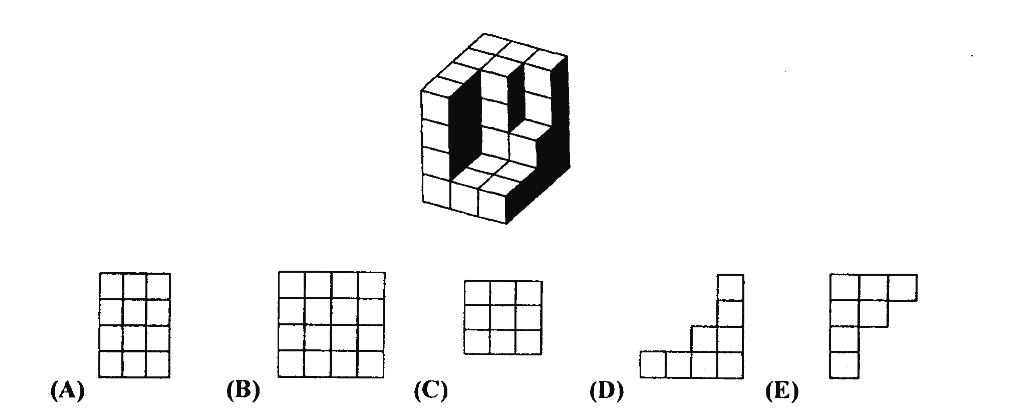
\includegraphics[width=1\textwidth]{2008SAC26.PNG}
    \end{center}

    \item %% Problem 7
    Which of the following is not one of the fourth roots of $16(\cos 120\degree + i\sin 120\degree)$?

    $\textbf{(A)} -\sqrt{3}-i \qquad \textbf{(B)} \sqrt{3}+i \qquad \textbf{(C)} 1-\sqrt{3}i \qquad \textbf{(D)} -\sqrt{3}+i \qquad \textbf{(E)} -1+\sqrt{3}i$

    \item %% Problem 8
    Consider the sequence $17,21,25,29,33,37,\dots,129,133$. Find the sum of the terms of the sequence.

    \item %% Problem 9
    $ABC1_{16}+ABC1_{15}=\blank_{14}$

    \item %% Problem 10
    
\end{enumerate}

\section*{Solutions}
\begin{enumerate}[label=\bfseries\arabic*.]
    \item %% Problem 1
    Associative 

    \item %% Problem 2
    not a function 

    \item %% Problem 3
    C 

    \item %% Problem 4
    1 

    \item %% Problem 5
    even function 

    \item %% Problem 6
    A 

    \item %% Problem 7
    D 

    \item %% Problem 8
    2250

    \item %% Problem 9
    21411

    \item %% Problem 10
    
\end{enumerate}

\end{document}